\chapter{Formalizing claims}

This chapter is about formalizing claims. \\
this should contain the microstructure approach and the ontology approach \\

\section{Microstructures}

\begin{figure}
	\begin{center}
      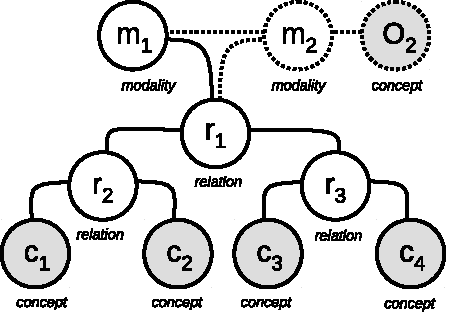
\includegraphics[scale=1]{microstructure.pdf}
      \end{center}
      \caption{Claim microstructure (2nd-order).}
  \label{fig:structures_flowchart}
\end{figure}

- microstructures are structures expressing relations between the domain-specific
concepts, reflecting beliefs, value judgements, or desired policies of the claim
author \\
- their purpose is to capture the gist of the claim \\
- they stemmed from as many claims could be expressed as a \emph{relation} between \emph{concepts} using 
a certain \emph{modality} \\
- figure~\ref{fig:structures_flowchart} shows a claim microstructure bringing three elements 
together \\

\noindent - Relations.  \\
- Many claims can be represented as expressing a relation between two concepts \\
- for example, on the topic of ``Gay Rights'' , the relations may be 
`\texttt{promotes(gay marriage, depopulation)}' and 
`\texttt{purpose(love, procreation)}' \\
- there are also comparably fewer claims that can be expressed via
higher-order relations , e.g. `\texttt{entails(constitution, allow(state, gay marriage))} \\
- each relation can be negated, e.g. $\neg$\texttt{promotes(gay marriage, depopulation)} expresses
that gay marriage does not cause depopulation \\
- relations are domain independent \\

\noindent Concepts \\
- the relations are established between concepts, expressed by noun phrases \\
- for ease of access, they can be arranged into a small, domain specific taxonomy of concepts \\
- for instance ``gay marriage'', ``heterosexual marriage'' and ``religious marriage''
all belong under the concept of ``marrriage'' \\
- the taxonomic relations could also be useful for later computational processing \\
- concepts are domain dependent and need to defined for each topic anew \\

\noindent Modalities \\
- we observe that claims are expressed under different modalities \\
- they can be roughly categorized into \textit{beliefs, value judgements, and policies} \\
- we formalize this via unary relations `believes', `approves', `disapproves', and `desires' corresponding 
to beliefs (factual, religous, and opinion-based), positive value judgements, negative value 
judgements, and desired policy (desired state of affairs) respectively \\
- the three modalities act as a wrapper on the propositional content of the claim, 
effectively modulating what is being claimed \\
- for instance, `\texttt{believes(purpose(love, procreation))}' expresses the belief 
that love serves procreation, while \texttt{desires(}$\neg$\texttt{allow(state, gay marriage))}'
expresses the wish for the state not to allow gay marriages \\
- finally, in a number of claims the claim is expressed with a reference to a second
opinion holder (e.g. the Bible, the state) \\
- to tackle this, we add an additional modality layer with the opinion holder as
an additional modifier \\
- for instance `\texttt{believes(believes[state](promotes(marriage, advancement)))}' corresponds
to the belief that the state believes gay marriages lead to an advancement \\
- by convention , the opinion holder of the first modality is always the author of the post \\

\begin{table}
{\footnotesize
\begin{tabular}{lp{0.80\columnwidth}}
\toprule
\textbf{Relation} & \textbf{Definition} \\
\midrule
\texttt{promotes(A, B)} & Promoting agent A promotes, fosters, leads, increases likelihood, boosts B.  \\
\texttt{suppress(A, B)} & Suppressing agent A suppresses, decreases likelihood, puts down, vanquishes B \\
\midrule
\texttt{allow(A, B)} & Principle A allows, approves, licenses state of affairs B \\
\midrule
\texttt{entails(A, B)} & State of affairs A, necessarily, per definition or causally, makes B true. \\
\texttt{contradicts(A, B)} & State of affairs A, necessarily, per definition or causally, makes B false. \\
\midrule
\texttt{purpose(A, B)} & The purpose of A is B. \\
\midrule
\texttt{equal(A, B)} & State of affairs A is equal to state of affairs B. \\
\midrule
\texttt{has(A, B)} & A has the properties affected by the existence of B.  \\
\bottomrule
\end{tabular}}
\caption{Relation types in claim microstructures.}
\label{tab:microstructures_relations}
\end{table}

\noindent - $\mathcal{R}, \mathcal{C}$, and $\mathcal{M}$ denote the set of relations, concepts and
modalities, respectively \\
- we define a claim microstructure as a quadruple 
$$
(m_1, m_2, o_2, r)
$$ 
where $m_1 \in \mathcal{M}$, and (optionally) $m_2 \in \mathcal{M} \cup \{\epsilon\}$,
$o_2 \in \mathcal{C} \cup \{\epsilon\}$ is the optional second opinion holder, and 
$r = (t, c_1, c_2) \in \mathcal{R}$ is the (possibly higher order) relation 
between two concepts or relations $c_1, c_2 \in \mathcal{C} \cup \mathcal{R}$, 
conveyed by the relation type $t$. \\
- table~\ref{tab:microstructures_relations} lists all possible relation types \\
